\documentclass[a4paper]{article}
\usepackage[a4paper,left=3cm,right=2cm,top=2.5cm,bottom=2.5cm]{geometry}
\usepackage{palatino}
\usepackage[colorlinks=true,linkcolor=blue,citecolor=blue]{hyperref}
\usepackage{graphicx}
\usepackage{cp1718t}
\usepackage{subcaption}
\usepackage{adjustbox}
%================= lhs2tex=====================================================%
%% ODER: format ==         = "\mathrel{==}"
%% ODER: format /=         = "\neq "
%
%
\makeatletter
\@ifundefined{lhs2tex.lhs2tex.sty.read}%
  {\@namedef{lhs2tex.lhs2tex.sty.read}{}%
   \newcommand\SkipToFmtEnd{}%
   \newcommand\EndFmtInput{}%
   \long\def\SkipToFmtEnd#1\EndFmtInput{}%
  }\SkipToFmtEnd

\newcommand\ReadOnlyOnce[1]{\@ifundefined{#1}{\@namedef{#1}{}}\SkipToFmtEnd}
\usepackage{amstext}
\usepackage{amssymb}
\usepackage{stmaryrd}
\DeclareFontFamily{OT1}{cmtex}{}
\DeclareFontShape{OT1}{cmtex}{m}{n}
  {<5><6><7><8>cmtex8
   <9>cmtex9
   <10><10.95><12><14.4><17.28><20.74><24.88>cmtex10}{}
\DeclareFontShape{OT1}{cmtex}{m}{it}
  {<-> ssub * cmtt/m/it}{}
\newcommand{\texfamily}{\fontfamily{cmtex}\selectfont}
\DeclareFontShape{OT1}{cmtt}{bx}{n}
  {<5><6><7><8>cmtt8
   <9>cmbtt9
   <10><10.95><12><14.4><17.28><20.74><24.88>cmbtt10}{}
\DeclareFontShape{OT1}{cmtex}{bx}{n}
  {<-> ssub * cmtt/bx/n}{}
\newcommand{\tex}[1]{\text{\texfamily#1}}	% NEU

\newcommand{\Sp}{\hskip.33334em\relax}


\newcommand{\Conid}[1]{\mathit{#1}}
\newcommand{\Varid}[1]{\mathit{#1}}
\newcommand{\anonymous}{\kern0.06em \vbox{\hrule\@width.5em}}
\newcommand{\plus}{\mathbin{+\!\!\!+}}
\newcommand{\bind}{\mathbin{>\!\!\!>\mkern-6.7mu=}}
\newcommand{\rbind}{\mathbin{=\mkern-6.7mu<\!\!\!<}}% suggested by Neil Mitchell
\newcommand{\sequ}{\mathbin{>\!\!\!>}}
\renewcommand{\leq}{\leqslant}
\renewcommand{\geq}{\geqslant}
\usepackage{polytable}

%mathindent has to be defined
\@ifundefined{mathindent}%
  {\newdimen\mathindent\mathindent\leftmargini}%
  {}%

\def\resethooks{%
  \global\let\SaveRestoreHook\empty
  \global\let\ColumnHook\empty}
\newcommand*{\savecolumns}[1][default]%
  {\g@addto@macro\SaveRestoreHook{\savecolumns[#1]}}
\newcommand*{\restorecolumns}[1][default]%
  {\g@addto@macro\SaveRestoreHook{\restorecolumns[#1]}}
\newcommand*{\aligncolumn}[2]%
  {\g@addto@macro\ColumnHook{\column{#1}{#2}}}

\resethooks

\newcommand{\onelinecommentchars}{\quad-{}- }
\newcommand{\commentbeginchars}{\enskip\{-}
\newcommand{\commentendchars}{-\}\enskip}

\newcommand{\visiblecomments}{%
  \let\onelinecomment=\onelinecommentchars
  \let\commentbegin=\commentbeginchars
  \let\commentend=\commentendchars}

\newcommand{\invisiblecomments}{%
  \let\onelinecomment=\empty
  \let\commentbegin=\empty
  \let\commentend=\empty}

\visiblecomments

\newlength{\blanklineskip}
\setlength{\blanklineskip}{0.66084ex}

\newcommand{\hsindent}[1]{\quad}% default is fixed indentation
\let\hspre\empty
\let\hspost\empty
\newcommand{\NB}{\textbf{NB}}
\newcommand{\Todo}[1]{$\langle$\textbf{To do:}~#1$\rangle$}

\EndFmtInput
\makeatother
%
%
%
%
%
%
% This package provides two environments suitable to take the place
% of hscode, called "plainhscode" and "arrayhscode". 
%
% The plain environment surrounds each code block by vertical space,
% and it uses \abovedisplayskip and \belowdisplayskip to get spacing
% similar to formulas. Note that if these dimensions are changed,
% the spacing around displayed math formulas changes as well.
% All code is indented using \leftskip.
%
% Changed 19.08.2004 to reflect changes in colorcode. Should work with
% CodeGroup.sty.
%
\ReadOnlyOnce{polycode.fmt}%
\makeatletter

\newcommand{\hsnewpar}[1]%
  {{\parskip=0pt\parindent=0pt\par\vskip #1\noindent}}

% can be used, for instance, to redefine the code size, by setting the
% command to \small or something alike
\newcommand{\hscodestyle}{}

% The command \sethscode can be used to switch the code formatting
% behaviour by mapping the hscode environment in the subst directive
% to a new LaTeX environment.

\newcommand{\sethscode}[1]%
  {\expandafter\let\expandafter\hscode\csname #1\endcsname
   \expandafter\let\expandafter\endhscode\csname end#1\endcsname}

% "compatibility" mode restores the non-polycode.fmt layout.

\newenvironment{compathscode}%
  {\par\noindent
   \advance\leftskip\mathindent
   \hscodestyle
   \let\\=\@normalcr
   \let\hspre\(\let\hspost\)%
   \pboxed}%
  {\endpboxed\)%
   \par\noindent
   \ignorespacesafterend}

\newcommand{\compaths}{\sethscode{compathscode}}

% "plain" mode is the proposed default.
% It should now work with \centering.
% This required some changes. The old version
% is still available for reference as oldplainhscode.

\newenvironment{plainhscode}%
  {\hsnewpar\abovedisplayskip
   \advance\leftskip\mathindent
   \hscodestyle
   \let\hspre\(\let\hspost\)%
   \pboxed}%
  {\endpboxed%
   \hsnewpar\belowdisplayskip
   \ignorespacesafterend}

\newenvironment{oldplainhscode}%
  {\hsnewpar\abovedisplayskip
   \advance\leftskip\mathindent
   \hscodestyle
   \let\\=\@normalcr
   \(\pboxed}%
  {\endpboxed\)%
   \hsnewpar\belowdisplayskip
   \ignorespacesafterend}

% Here, we make plainhscode the default environment.

\newcommand{\plainhs}{\sethscode{plainhscode}}
\newcommand{\oldplainhs}{\sethscode{oldplainhscode}}
\plainhs

% The arrayhscode is like plain, but makes use of polytable's
% parray environment which disallows page breaks in code blocks.

\newenvironment{arrayhscode}%
  {\hsnewpar\abovedisplayskip
   \advance\leftskip\mathindent
   \hscodestyle
   \let\\=\@normalcr
   \(\parray}%
  {\endparray\)%
   \hsnewpar\belowdisplayskip
   \ignorespacesafterend}

\newcommand{\arrayhs}{\sethscode{arrayhscode}}

% The mathhscode environment also makes use of polytable's parray 
% environment. It is supposed to be used only inside math mode 
% (I used it to typeset the type rules in my thesis).

\newenvironment{mathhscode}%
  {\parray}{\endparray}

\newcommand{\mathhs}{\sethscode{mathhscode}}

% texths is similar to mathhs, but works in text mode.

\newenvironment{texthscode}%
  {\(\parray}{\endparray\)}

\newcommand{\texths}{\sethscode{texthscode}}

% The framed environment places code in a framed box.

\def\codeframewidth{\arrayrulewidth}
\RequirePackage{calc}

\newenvironment{framedhscode}%
  {\parskip=\abovedisplayskip\par\noindent
   \hscodestyle
   \arrayrulewidth=\codeframewidth
   \tabular{@{}|p{\linewidth-2\arraycolsep-2\arrayrulewidth-2pt}|@{}}%
   \hline\framedhslinecorrect\\{-1.5ex}%
   \let\endoflinesave=\\
   \let\\=\@normalcr
   \(\pboxed}%
  {\endpboxed\)%
   \framedhslinecorrect\endoflinesave{.5ex}\hline
   \endtabular
   \parskip=\belowdisplayskip\par\noindent
   \ignorespacesafterend}

\newcommand{\framedhslinecorrect}[2]%
  {#1[#2]}

\newcommand{\framedhs}{\sethscode{framedhscode}}

% The inlinehscode environment is an experimental environment
% that can be used to typeset displayed code inline.

\newenvironment{inlinehscode}%
  {\(\def\column##1##2{}%
   \let\>\undefined\let\<\undefined\let\\\undefined
   \newcommand\>[1][]{}\newcommand\<[1][]{}\newcommand\\[1][]{}%
   \def\fromto##1##2##3{##3}%
   \def\nextline{}}{\) }%

\newcommand{\inlinehs}{\sethscode{inlinehscode}}

% The joincode environment is a separate environment that
% can be used to surround and thereby connect multiple code
% blocks.

\newenvironment{joincode}%
  {\let\orighscode=\hscode
   \let\origendhscode=\endhscode
   \def\endhscode{\def\hscode{\endgroup\def\@currenvir{hscode}\\}\begingroup}
   %\let\SaveRestoreHook=\empty
   %\let\ColumnHook=\empty
   %\let\resethooks=\empty
   \orighscode\def\hscode{\endgroup\def\@currenvir{hscode}}}%
  {\origendhscode
   \global\let\hscode=\orighscode
   \global\let\endhscode=\origendhscode}%

\makeatother
\EndFmtInput
%
\def\ana#1{\mathopen{[\!(}#1\mathclose{)\!]}}

%---------------------------------------------------------------------------

\title{
       	    Cálculo de Programas
\\
       	Trabalho Prático
\\
       	MiEI+LCC --- 2017/18
}

\author{
       	\dium
\\
       	Universidade do Minho
}


\date\mydate

\makeindex

\begin{document}

\maketitle

\begin{center}\large
\begin{tabular}{ll}
\textbf{Grupo} nr. & 99 (preencher)
\\\hline
a11111 & Nome1 (preencher)	
\\
a22222 & Nome2 (preencher)	
\\
a33333 & Nome3 (preencher)	
\end{tabular}
\end{center}

\section{Preâmbulo}

A disciplina de \CP\ tem como objectivo principal ensinar
a progra\-mação de computadores como uma disciplina científica. Para isso
parte-se de um repertório de \emph{combinadores} que formam uma álgebra da
programação (conjunto de leis universais e seus corolários) e usam-se esses
combinadores para construir programas \emph{composicionalmente}, isto é,
agregando programas já existentes.
  
Na sequência pedagógica dos planos de estudo dos dois cursos que têm esta
disciplina, restringe-se a aplicação deste método à programação funcional
em \Haskell. Assim, 
o presente trabalho prático coloca os alunos perante problemas
concretos que deverão ser implementados em \Haskell.
Há ainda um outro objectivo: o de ensinar a documentar programas e
a produzir textos técnico-científicos de qualidade.

\section{Documentação}
Para cumprir de forma integrada os objectivos enunciados acima vamos recorrer
a uma técnica de programa\-ção dita ``\litp{literária}'' \cite{Kn92}, cujo
princípio base é o seguinte:
\begin{quote}\em
Um programa e a sua documentação devem coincidir.
\end{quote}
Por outras palavras, o código fonte e a documentação de um programa deverão estar no
mesmo ficheiro.

O ficheiro \texttt{cp1718t.pdf} que está a ler é já um exemplo de \litp{programação
literária}: foi gerado a partir do texto fonte \texttt{cp1718t.lhs}\footnote{O
suffixo `lhs' quer dizer \emph{\lhaskell{literate Haskell}}.} que encontrará
no \MaterialPedagogico\ desta disciplina descompactando o ficheiro \texttt{cp1718t.zip}
e executando
\begin{Verbatim}[fontsize=\small]
    $ lhs2TeX cp1718t.lhs > cp1718t.tex
    $ pdflatex cp1718t
\end{Verbatim}
em que \href{https://hackage.haskell.org/package/lhs2tex}{\texttt\LhsToTeX} é
um pre-processador que faz ``pretty printing''
de código Haskell em \Latex\ e que deve desde já instalar executando
\begin{Verbatim}[fontsize=\small]
    $ cabal install lhs2tex
\end{Verbatim}
Por outro lado, o mesmo ficheiro \texttt{cp1718t.lhs} é executável e contém
o ``kit'' básico, escrito em \Haskell, para realizar o trabalho. Basta executar
\begin{Verbatim}[fontsize=\small]
    $ ghci cp1718t.lhs
\end{Verbatim}


\noindent Abra o ficheiro \texttt{cp1718t.lhs} no seu editor de texto preferido
e verifique que assim é: todo o texto que se encontra dentro do ambiente
\begin{quote}\small\tt
\text{\ttfamily \char92{}begin\char123{}code\char125{}}
\\ ... \\
\text{\ttfamily \char92{}end\char123{}code\char125{}}
\end{quote}
vai ser seleccionado pelo \GHCi\ para ser executado.

\section{Como realizar o trabalho}
Este trabalho teórico-prático deve ser realizado por grupos de três alunos.
Os detalhes da avaliação (datas para submissão do relatório e sua defesa
oral) são os que forem publicados na \cp{página da disciplina} na \emph{internet}.

Recomenda-se uma abordagem participativa dos membros do grupo
de trabalho por forma a poderem responder às questões que serão colocadas
na \emph{defesa oral} do relatório.

Em que consiste, então, o \emph{relatório} a que se refere o parágrafo anterior?
É a edição do texto que está a ser lido, preenchendo o anexo \ref{sec:resolucao}
com as respostas. O relatório deverá conter ainda a identificação dos membros
do grupo de trabalho, no local respectivo da folha de rosto.

Para gerar o PDF integral do relatório deve-se ainda correr os comando seguintes,
que actualizam a bibliografia (com \Bibtex) e o índice remissivo (com \Makeindex),
\begin{Verbatim}[fontsize=\small]
    $ bibtex cp1718t.aux
    $ makeindex cp1718t.idx
\end{Verbatim}
e recompilar o texto como acima se indicou. Dever-se-á ainda instalar o utilitário
\QuickCheck,
que ajuda a validar programas em \Haskell, a biblioteca
\href{https://hackage.haskell.org/package/JuicyPixels}{JuicyPixels} para processamento
de imagens e a biblioteca \href{http://gloss.ouroborus.net/}{gloss} para geração de gráficos 2D:
\begin{Verbatim}[fontsize=\small]
    $ cabal install QuickCheck JuicyPixels gloss
\end{Verbatim}
Para testar uma propriedade \QuickCheck~\ensuremath{\Varid{prop}}, basta invocá-la com o comando:
\begin{tabbing}\ttfamily
~~~~~\char62{}~quickCheck~prop\\
\ttfamily ~~~~~\char43{}\char43{}\char43{}~OK\char44{}~passed~100~tests\char46{}
\end{tabbing}

\section*{Problema 1}

Segundo uma \href{https://www.jn.pt/economia/interior/compra-diaria-de-bitcoins-iguala-acoes-da-apple-9257302.html}{notícia do Jornal de Notícias}, 
referente ao dia 12 de abril, \emph{``apenas numa hora, foram transacionadas 1.2 mil milhões de dólares em bitcoins. Nas últimas 24 horas, foram transacionados 8,5 mil milhões de dólares, num total de 24 mil milhões de dólares referentes às principais criptomoedas''}.

De facto, é inquestionável que as criptomoedas, e em particular as bitcoin, vieram para ficar.
%
Várias moedas digitais, e em particular as bitcoin, usam a tecnologia de block chain
para guardar e assegurar todas as transações relacionadas com a moeda.
%
Uma \href{https://en.bitcoin.it/wiki/Block_chain}{block chain} é uma coleção de blocos que registam os movimentos da moeda; a sua definição em Haskell é apresentada de seguida.

\begin{hscode}\SaveRestoreHook
\column{B}{@{}>{\hspre}l<{\hspost}@{}}%
\column{37}{@{}>{\hspre}c<{\hspost}@{}}%
\column{37E}{@{}l@{}}%
\column{40}{@{}>{\hspre}l<{\hspost}@{}}%
\column{E}{@{}>{\hspre}l<{\hspost}@{}}%
\>[B]{}\mathbf{data}\;\Conid{Blockchain}\mathrel{=}\Conid{Bc}\;\{\mskip1.5mu \Varid{bc}\mathbin{::}\Conid{Block}\mskip1.5mu\}{}\<[37]%
\>[37]{}\mid {}\<[37E]%
\>[40]{}\Conid{Bcs}\;\{\mskip1.5mu \Varid{bcs}\mathbin{::}(\Conid{Block},\Conid{Blockchain})\mskip1.5mu\}\;\mathbf{deriving}\;\Conid{Show}{}\<[E]%
\ColumnHook
\end{hscode}\resethooks

Cada \href{https://en.bitcoin.it/wiki/Block}{bloco} numa block chain
regista um número (mágico) único, o momento da execução, e uma lista de transações,
tal como no código seguinte:

\begin{hscode}\SaveRestoreHook
\column{B}{@{}>{\hspre}l<{\hspost}@{}}%
\column{E}{@{}>{\hspre}l<{\hspost}@{}}%
\>[B]{}\mathbf{type}\;\Conid{Block}\mathrel{=}(\Conid{MagicNo},(\Conid{Time},\Conid{Transactions})){}\<[E]%
\ColumnHook
\end{hscode}\resethooks

Cada \href{https://en.bitcoin.it/wiki/Transaction}{transação} 
define a entidade de origem da transferência, o valor a ser transacionado,
e a entidade destino (por esta ordem), tal como se define de seguida.

\begin{hscode}\SaveRestoreHook
\column{B}{@{}>{\hspre}l<{\hspost}@{}}%
\column{E}{@{}>{\hspre}l<{\hspost}@{}}%
\>[B]{}\mathbf{type}\;\Conid{Transaction}\mathrel{=}(\Conid{Entity},(\Conid{Value},\Conid{Entity})){}\<[E]%
\\
\>[B]{}\mathbf{type}\;\Conid{Transactions}\mathrel{=}[\mskip1.5mu \Conid{Transaction}\mskip1.5mu]{}\<[E]%
\ColumnHook
\end{hscode}\resethooks

A partir de uma block chain, é possível calcular o valor que cada entidade
detém, tipicamente designado de ledger:

\begin{hscode}\SaveRestoreHook
\column{B}{@{}>{\hspre}l<{\hspost}@{}}%
\column{E}{@{}>{\hspre}l<{\hspost}@{}}%
\>[B]{}\mathbf{type}\;\Conid{Ledger}\mathrel{=}[\mskip1.5mu (\Conid{Entity},\Conid{Value})\mskip1.5mu]{}\<[E]%
\ColumnHook
\end{hscode}\resethooks

Seguem as restantes definições Haskell para completar o código anterior.
Note que \ensuremath{\Conid{Time}} representa o momento da transação, como o número de \href{https://currentmillis.com}{milisegundos} que passaram desde 1970.

\begin{hscode}\SaveRestoreHook
\column{B}{@{}>{\hspre}l<{\hspost}@{}}%
\column{18}{@{}>{\hspre}l<{\hspost}@{}}%
\column{E}{@{}>{\hspre}l<{\hspost}@{}}%
\>[B]{}\mathbf{type}\;\Conid{MagicNo}\mathrel{=}\Conid{String}{}\<[E]%
\\
\>[B]{}\mathbf{type}\;\Conid{Time}\mathrel{=}\Conid{Int}{}\<[18]%
\>[18]{}\mbox{\onelinecomment  em milisegundos}{}\<[E]%
\\
\>[B]{}\mathbf{type}\;\Conid{Entity}\mathrel{=}\Conid{String}{}\<[E]%
\\
\>[B]{}\mathbf{type}\;\Conid{Value}\mathrel{=}\Conid{Int}{}\<[E]%
\ColumnHook
\end{hscode}\resethooks

Neste contexto, implemente as seguintes funções:

\begin{enumerate}
\item Defina a função \ensuremath{\Varid{allTransactions}\mathbin{::}\Conid{Blockchain}\to \Conid{Transactions}}, como um catamorfismo, que calcula a lista com todas as transações numa dada block chain.


\begin{propriedade}
    As transações de uma block chain são as mesmas da block chain revertida:
\begin{hscode}\SaveRestoreHook
\column{B}{@{}>{\hspre}l<{\hspost}@{}}%
\column{E}{@{}>{\hspre}l<{\hspost}@{}}%
\>[B]{}\Varid{prop1a}\mathrel{=}\Varid{sort}\comp \Varid{allTransactions}\equiv\Varid{sort}\comp \Varid{allTransactions}\comp \Varid{reverseChain}{}\<[E]%
\ColumnHook
\end{hscode}\resethooks

Note que a função \ensuremath{\Varid{sort}} é usada apenas para facilitar a comparação das listas.
\end{propriedade}

\item Defina a função \ensuremath{\Varid{ledger}\mathbin{::}\Conid{Blockchain}\to \Conid{Ledger}}, utilizando catamorfismos e/ou anamorfismos, que calcula o ledger (i.e., o valor disponível) de cada entidade numa uma dada block chain.
    Note que as entidades podem ter valores negativos; de facto isso acontecerá para a primeira transação que executarem.


\begin{propriedade}
    O tamanho do ledger é inferior ou igual a duas vezes o tamanho de todas as transações:
\begin{hscode}\SaveRestoreHook
\column{B}{@{}>{\hspre}l<{\hspost}@{}}%
\column{E}{@{}>{\hspre}l<{\hspost}@{}}%
\>[B]{}\Varid{prop1b}\mathrel{=}\length \comp \Varid{ledger}\leq(\mathrm{2}\mathbin{*})\comp \length \comp \Varid{allTransactions}{}\<[E]%
\ColumnHook
\end{hscode}\resethooks
\end{propriedade}

\begin{propriedade}
    O ledger de uma block chain é igual ao ledger da sua inversa:
\begin{hscode}\SaveRestoreHook
\column{B}{@{}>{\hspre}l<{\hspost}@{}}%
\column{E}{@{}>{\hspre}l<{\hspost}@{}}%
\>[B]{}\Varid{prop1c}\mathrel{=}\Varid{sort}\comp \Varid{ledger}\equiv\Varid{sort}\comp \Varid{ledger}\comp \Varid{reverseChain}{}\<[E]%
\ColumnHook
\end{hscode}\resethooks
\end{propriedade}



\item Defina a função \ensuremath{\Varid{isValidMagicNr}\mathbin{::}\Conid{Blockchain}\to \Conid{Bool}}, utilizando catamorfismos e/ou anamorfismos, que verifica se todos os números mágicos numa dada block chain são únicos.


\begin{propriedade}
    A concatenação de uma block chain com ela mesma nunca é válida em termos de números mágicos:
\begin{hscode}\SaveRestoreHook
\column{B}{@{}>{\hspre}l<{\hspost}@{}}%
\column{E}{@{}>{\hspre}l<{\hspost}@{}}%
\>[B]{}\Varid{prop1d}\mathrel{=}\neg \comp \Varid{isValidMagicNr}\comp \Varid{concChain}\comp \conj{\Varid{id}}{\Varid{id}}{}\<[E]%
\ColumnHook
\end{hscode}\resethooks
\end{propriedade}

\begin{propriedade}
    Se uma block chain é válida em termos de números mágicos, então a sua inversa também o é:
\begin{hscode}\SaveRestoreHook
\column{B}{@{}>{\hspre}l<{\hspost}@{}}%
\column{E}{@{}>{\hspre}l<{\hspost}@{}}%
\>[B]{}\Varid{prop1e}\mathrel{=}\Varid{isValidMagicNr}\Rightarrow\Varid{isValidMagicNr}\comp \Varid{reverseChain}{}\<[E]%
\ColumnHook
\end{hscode}\resethooks
\end{propriedade}

\end{enumerate}



\section*{Problema 2}

Uma estrutura de dados frequentemente utilizada para representação e processamento de imagens de forma eficiente são as denominadas \href{https://en.wikipedia.org/wiki/Quadtree}{quadtrees}.
Uma \emph{quadtree} é uma árvore quaternária em que cada nodo tem quatro sub-árvores e cada folha representa um valor bi-dimensional.
\begin{hscode}\SaveRestoreHook
\column{B}{@{}>{\hspre}l<{\hspost}@{}}%
\column{3}{@{}>{\hspre}l<{\hspost}@{}}%
\column{E}{@{}>{\hspre}l<{\hspost}@{}}%
\>[B]{}\mathbf{data}\;\Conid{QTree}\;\Varid{a}\mathrel{=}\Conid{Cell}\;\Varid{a}\;\Conid{Int}\;\Conid{Int}\mid \Conid{Block}\;(\Conid{QTree}\;\Varid{a})\;(\Conid{QTree}\;\Varid{a})\;(\Conid{QTree}\;\Varid{a})\;(\Conid{QTree}\;\Varid{a}){}\<[E]%
\\
\>[B]{}\hsindent{3}{}\<[3]%
\>[3]{}\mathbf{deriving}\;(\Conid{Eq},\Conid{Show}){}\<[E]%
\ColumnHook
\end{hscode}\resethooks

\begin{figure}
\begin{subfigure}{0.3\textwidth}
\begin{tabbing}\ttfamily
~\char40{}~0~0~0~0~0~0~0~0~\char41{}\\
\ttfamily ~\char40{}~0~0~0~0~0~0~0~0~\char41{}\\
\ttfamily ~\char40{}~0~0~0~0~1~1~1~0~\char41{}\\
\ttfamily ~\char40{}~0~0~0~0~1~1~0~0~\char41{}\\
\ttfamily ~\char40{}~1~1~1~1~1~1~0~0~\char41{}\\
\ttfamily ~\char40{}~1~1~1~1~1~1~0~0~\char41{}\\
\ttfamily ~\char40{}~1~1~1~1~0~0~0~0~\char41{}\\
\ttfamily ~\char40{}~1~1~1~1~0~0~0~1~\char41{}
\end{tabbing}
\caption{Matriz de exemplo \ensuremath{\Varid{bm}}.}
\label{fig:bm}
\end{subfigure}
\begin{subfigure}{0.7\textwidth}
\begin{tabbing}\ttfamily
~Block\\
\ttfamily ~~\char40{}Cell~0~4~4\char41{}~\char40{}Block\\
\ttfamily ~~~\char40{}Cell~0~2~2\char41{}~\char40{}Cell~0~2~2\char41{}~\char40{}Cell~1~2~2\char41{}~\char40{}Block\\
\ttfamily ~~~~\char40{}Cell~1~1~1\char41{}~\char40{}Cell~0~1~1\char41{}~\char40{}Cell~0~1~1\char41{}~\char40{}Cell~0~1~1\char41{}\char41{}\char41{}\\
\ttfamily ~~\char40{}Cell~1~4~4\char41{}\\
\ttfamily ~~\char40{}Block\\
\ttfamily ~~~\char40{}Cell~1~2~2\char41{}~\char40{}Cell~0~2~2\char41{}~\char40{}Cell~0~2~2\char41{}~\char40{}Block\\
\ttfamily ~~~~\char40{}Cell~0~1~1\char41{}~\char40{}Cell~0~1~1\char41{}~\char40{}Cell~0~1~1\char41{}~\char40{}Cell~1~1~1\char41{}\char41{}\char41{}
\end{tabbing}
\caption{Quadtree de exemplo \ensuremath{\Varid{qt}}.}
\label{fig:qt}
\end{subfigure}
\caption{Exemplos de representações de bitmaps.}
\end{figure}

Uma imagem monocromática em formato bitmap pode ser representada como uma
matriz de bits\footnote{Cf.\ módulo \href{https://hackage.haskell.org/package/matrix}{\ensuremath{\Conid{\Conid{Data}.Matrix}}}.},
tal como se exemplifica na Figura~\ref{fig:bm}.

O anamorfismo \ensuremath{\Varid{bm2qt}} converte um bitmap em forma matricial na sua codificação eficiente em quadtrees, e o catamorfismo \ensuremath{\Varid{qt2bm}} executa a operação inversa:

\adjustbox{valign=t}{\begin{minipage}{.5\textwidth} %
\begingroup
\leftskip-1.5em
\rightskip\leftskip
\begin{hscode}\SaveRestoreHook
\column{B}{@{}>{\hspre}l<{\hspost}@{}}%
\column{5}{@{}>{\hspre}l<{\hspost}@{}}%
\column{6}{@{}>{\hspre}l<{\hspost}@{}}%
\column{13}{@{}>{\hspre}l<{\hspost}@{}}%
\column{E}{@{}>{\hspre}l<{\hspost}@{}}%
\>[B]{}\Varid{bm2qt}\mathbin{::}(\Conid{Eq}\;\Varid{a})\Rightarrow \Conid{Matrix}\;\Varid{a}\to \Conid{QTree}\;\Varid{a}{}\<[E]%
\\
\>[B]{}\Varid{bm2qt}\mathrel{=}\Varid{anaQTree}\;\Varid{f}\;\mathbf{where}{}\<[E]%
\\
\>[B]{}\hsindent{5}{}\<[5]%
\>[5]{}\Varid{f}\;\Varid{m}\mathrel{=}\mathbf{if}\;\Varid{one}\;\mathbf{then}\;i_1\;\Varid{u}\;\mathbf{else}\;i_2\;(\Varid{a},(\Varid{b},(\Varid{c},\Varid{d}))){}\<[E]%
\\
\>[5]{}\hsindent{1}{}\<[6]%
\>[6]{}\mathbf{where}\;{}\<[13]%
\>[13]{}\Varid{x}\mathrel{=}(\Varid{nub}\comp \Varid{toList})\;\Varid{m}{}\<[E]%
\\
\>[13]{}\Varid{u}\mathrel{=}(\Varid{head}\;\Varid{x},(\Varid{ncols}\;\Varid{m},\Varid{nrows}\;\Varid{m})){}\<[E]%
\\
\>[13]{}\Varid{one}\mathrel{=}(\Varid{ncols}\;\Varid{m}\equiv \mathrm{1}\mathrel{\vee}\Varid{nrows}\;\Varid{m}\equiv \mathrm{1}\mathrel{\vee}\length \;\Varid{x}\equiv \mathrm{1}){}\<[E]%
\\
\>[13]{}(\Varid{a},\Varid{b},\Varid{c},\Varid{d})\mathrel{=}\Varid{splitBlocks}\;(\Varid{nrows}\;\Varid{m}\mathbin{\Varid{`div`}}\mathrm{2})\;(\Varid{ncols}\;\Varid{m}\mathbin{\Varid{`div`}}\mathrm{2})\;\Varid{m}{}\<[E]%
\ColumnHook
\end{hscode}\resethooks
\endgroup
\end{minipage}} %
\adjustbox{valign=t}{\begin{minipage}{.5\textwidth} %
\begingroup
\leftskip-2em
\rightskip\leftskip
\begin{hscode}\SaveRestoreHook
\column{B}{@{}>{\hspre}l<{\hspost}@{}}%
\column{5}{@{}>{\hspre}l<{\hspost}@{}}%
\column{E}{@{}>{\hspre}l<{\hspost}@{}}%
\>[B]{}\Varid{qt2bm}\mathbin{::}(\Conid{Eq}\;\Varid{a})\Rightarrow \Conid{QTree}\;\Varid{a}\to \Conid{Matrix}\;\Varid{a}{}\<[E]%
\\
\>[B]{}\Varid{qt2bm}\mathrel{=}\Varid{cataQTree}\;\alt{\Varid{f}}{\Varid{g}}\;\mathbf{where}{}\<[E]%
\\
\>[B]{}\hsindent{5}{}\<[5]%
\>[5]{}\Varid{f}\;(\Varid{k},(\Varid{i},\Varid{j}))\mathrel{=}matrix\;\Varid{j}\;\Varid{i}\;\underline{\Varid{k}}{}\<[E]%
\\
\>[B]{}\hsindent{5}{}\<[5]%
\>[5]{}\Varid{g}\;(\Varid{a},(\Varid{b},(\Varid{c},\Varid{d})))\mathrel{=}(\Varid{a}{\,\updownarrow\,}\Varid{b}){\,\leftrightarrow\,}(\Varid{c}{\,\updownarrow\,}\Varid{d}){}\<[E]%
\ColumnHook
\end{hscode}\resethooks
\endgroup
\end{minipage}}

O algoritmo \ensuremath{\Varid{bm2qt}} particiona recursivamente a imagem em $4$ blocos e termina produzindo folhas para matrizes unitárias ou quando todos os píxeis de um sub-bloco têm a mesma côr.
Para a matriz \ensuremath{\Varid{bm}} de exemplo, a quadtree correspondente \ensuremath{\Varid{qt}\mathrel{=}\Varid{bm2qt}\;\Varid{bm}} é ilustrada na Figura~\ref{fig:qt}.

\begin{figure}
%
\begin{subfigure}{0.5\textwidth}
\centering

\includegraphics[width=0.2\linewidth]{cp1718t_media/person.png}
\caption{Bitmap de exemplo.}
\label{fig:person}
\end{subfigure}
%
\begin{subfigure}{0.5\textwidth}
\centering

\includegraphics[height=0.2\linewidth]{cp1718t_media/person90.png}
\caption{Rotação.}
\label{fig:person90}
\end{subfigure}
%
\begin{subfigure}{0.5\textwidth}
\centering

\includegraphics[width=0.4\linewidth]{cp1718t_media/personx2.png}
\caption{Redimensionamento.}
\label{fig:personx2}
\end{subfigure}
%
\begin{subfigure}{0.5\textwidth}
\centering

\includegraphics[width=0.2\linewidth]{cp1718t_media/personinv.png}
\caption{Inversão de cores.}
\label{fig:personinv}
\end{subfigure}
%
\begin{subfigure}{0.5\textwidth}
\centering

\includegraphics[width=0.2\linewidth]{cp1718t_media/person1.png}
\caption{Compresão de $1$ nível.}
\label{fig:person1}
\end{subfigure}
%
\begin{subfigure}{0.5\textwidth}
\centering

\includegraphics[width=0.2\linewidth]{cp1718t_media/person2.png}
\caption{Compresão de $2$ níveis.}
\label{fig:person2}
\end{subfigure}
%
\begin{subfigure}{0.5\textwidth}
\centering

\includegraphics[width=0.2\linewidth]{cp1718t_media/person3.png}
\caption{Compresão de $3$ níveis.}
\label{fig:person3}
\end{subfigure}
%
\begin{subfigure}{0.5\textwidth}
\centering

\includegraphics[width=0.2\linewidth]{cp1718t_media/person4.png}
\caption{Compresão de $4$ níveis.}
\label{fig:person4}
\end{subfigure}
%
\begin{subfigure}{0.5\textwidth}
\centering

\includegraphics[width=0.2\linewidth]{cp1718t_media/personOut1.png}
\caption{Bitmap de contorno.}
\label{fig:personOut1}
\end{subfigure}
%
\begin{subfigure}{0.5\textwidth}
\centering

\includegraphics[width=0.2\linewidth]{cp1718t_media/personOut2.png}
\caption{Bitmap com contorno.}
\label{fig:personOut2}
\end{subfigure}
%
\caption{Manipulação de uma figura bitmap utilizando quadtrees.}
\end{figure}

Imagens a cores podem ser representadas como matrizes de píxeis segundo o código de cores \href{https://en.wikipedia.org/wiki/RGBA_color_space}{RGBA}, codificado no tipo \href{https://hackage.haskell.org/package/JuicyPixels-3.2.9.5/docs/Codec-Picture.html#t:PixelRGBA8}{\ensuremath{\Conid{PixelRGBA8}}} em que cada pixel é um quádruplo de valores inteiros $(red,green,blue,alpha)$ contidos entre $0$ e $255$.
Atente em alguns exemplos de cores:
\begin{hscode}\SaveRestoreHook
\column{B}{@{}>{\hspre}l<{\hspost}@{}}%
\column{10}{@{}>{\hspre}l<{\hspost}@{}}%
\column{E}{@{}>{\hspre}l<{\hspost}@{}}%
\>[B]{}\Varid{whitePx}{}\<[10]%
\>[10]{}\mathrel{=}\Conid{PixelRGBA8}\;\mathrm{255}\;\mathrm{255}\;\mathrm{255}\;\mathrm{255}{}\<[E]%
\\
\>[B]{}\Varid{blackPx}{}\<[10]%
\>[10]{}\mathrel{=}\Conid{PixelRGBA8}\;\mathrm{0}\;\mathrm{0}\;\mathrm{0}\;\mathrm{255}{}\<[E]%
\\
\>[B]{}\Varid{redPx}{}\<[10]%
\>[10]{}\mathrel{=}\Conid{PixelRGBA8}\;\mathrm{255}\;\mathrm{0}\;\mathrm{0}\;\mathrm{255}{}\<[E]%
\ColumnHook
\end{hscode}\resethooks

O módulo \ensuremath{\Conid{BMP}}, disponibilizado juntamente com o enunciado, fornece funções para processar ficheiros de imagem bitmap como matrizes:
\begin{hscode}\SaveRestoreHook
\column{B}{@{}>{\hspre}l<{\hspost}@{}}%
\column{5}{@{}>{\hspre}l<{\hspost}@{}}%
\column{E}{@{}>{\hspre}l<{\hspost}@{}}%
\>[5]{}\Varid{readBMP}\mathbin{::}\Conid{FilePath}\to \fun{IO}\;(\Conid{Matrix}\;\Conid{PixelRGBA8}){}\<[E]%
\\
\>[5]{}\Varid{writeBMP}\mathbin{::}\Conid{FilePath}\to \Conid{Matrix}\;\Conid{PixelRGBA8}\to \fun{IO}\;(){}\<[E]%
\ColumnHook
\end{hscode}\resethooks

Teste, por exemplo, no \ensuremath{\Conid{GHCi}}, carregar a Figura~\ref{fig:person}:
\begin{tabbing}\ttfamily
~~~~~\char62{}~readBMP~\char34{}cp1718t\char95{}media\char47{}person\char46{}bmp\char34{}
\end{tabbing}

Esta questão aborda operações de processamento de imagens utilizando quadtrees:
\begin{enumerate}
    \item Defina as funções \ensuremath{\Varid{rotateQTree}\mathbin{::}\Conid{QTree}\;\Varid{a}\to \Conid{QTree}\;\Varid{a}}, \ensuremath{\Varid{scaleQTree}\mathbin{::}\Conid{Int}\to \Conid{QTree}\;\Varid{a}\to \Conid{QTree}\;\Varid{a}} e \ensuremath{\Varid{invertQTree}\mathbin{::}\Conid{QTree}\;\Varid{a}\to \Conid{QTree}\;\Varid{a}}, como catamorfismos e/ou anamorfismos, que rodam\footnote{Segundo um ângulo de $90º$ no sentido dos ponteiros do relógio.}, redimensionam \footnote{Multiplicando o seu tamanho pelo valor recebido.} e invertem as cores de uma quadtree\footnote{Um pixel pode ser invertido calculando $255 - c$ para cada componente $c$ de cor RGB, exceptuando o componente alpha.}, respectivamente.
    Tente produzir imagens similares às Figuras~\ref{fig:person90}, \ref{fig:personx2} e \ref{fig:personinv}:
        \begin{tabbing}\ttfamily
~~~~~\char62{}~rotateBMP~~\char34{}cp1718t\char95{}media\char47{}person\char46{}bmp\char34{}~\char34{}person90\char46{}bmp\char34{}\\
\ttfamily ~~~~~\char62{}~scaleBMP~2~\char34{}cp1718t\char95{}media\char47{}person\char46{}bmp\char34{}~\char34{}personx2\char46{}bmp\char34{}\\
\ttfamily ~~~~~\char62{}~invertBMP~~\char34{}cp1718t\char95{}media\char47{}person\char46{}bmp\char34{}~\char34{}personinv\char46{}bmp\char34{}
\end{tabbing}

\begin{propriedade}
        Rodar uma quadtree é equivalente a rodar a matriz correspondente:
\begin{hscode}\SaveRestoreHook
\column{B}{@{}>{\hspre}l<{\hspost}@{}}%
\column{E}{@{}>{\hspre}l<{\hspost}@{}}%
\>[B]{}\Varid{prop2c}\mathrel{=}\Varid{rotateMatrix}\comp \Varid{qt2bm}\equiv\Varid{qt2bm}\comp \Varid{rotateQTree}{}\<[E]%
\ColumnHook
\end{hscode}\resethooks
    \end{propriedade}
\begin{propriedade}
    Redimensionar uma imagem altera o seu tamanho na mesma proporção:
\begin{hscode}\SaveRestoreHook
\column{B}{@{}>{\hspre}l<{\hspost}@{}}%
\column{E}{@{}>{\hspre}l<{\hspost}@{}}%
\>[B]{}\Varid{prop2d}\;(\Conid{Nat}\;\Varid{s})\mathrel{=}\Varid{sizeQTree}\comp \Varid{scaleQTree}\;\Varid{s}\equiv((\Varid{s}\mathbin{*})\times(\Varid{s}\mathbin{*}))\comp \Varid{sizeQTree}{}\<[E]%
\ColumnHook
\end{hscode}\resethooks
\end{propriedade}
\begin{propriedade}
    Inverter as cores de uma quadtree preserva a sua estrutura:
\begin{hscode}\SaveRestoreHook
\column{B}{@{}>{\hspre}l<{\hspost}@{}}%
\column{E}{@{}>{\hspre}l<{\hspost}@{}}%
\>[B]{}\Varid{prop2e}\mathrel{=}\Varid{shapeQTree}\comp \Varid{invertQTree}\equiv\Varid{shapeQTree}{}\<[E]%
\ColumnHook
\end{hscode}\resethooks
\end{propriedade}
    
    \item Defina a função \ensuremath{\Varid{compressQTree}\mathbin{::}\Conid{Int}\to \Conid{QTree}\;\Varid{a}\to \Conid{QTree}\;\Varid{a}}, utilizando catamorfismos e/ou anamorfismos, que comprime uma quadtree cortando folhas da árvore para reduzir a sua profundidade num dado número de níveis.
    Tente produzir imagens similares (mas não necessariamente iguais) às Figuras~\ref{fig:person1}, \ref{fig:person2}, \ref{fig:person3} e \ref{fig:person4}:
        \begin{tabbing}\ttfamily
~~~~~\char62{}~compressBMP~1~\char34{}cp1718t\char95{}media\char47{}person\char46{}bmp\char34{}~\char34{}person1\char46{}bmp\char34{}\\
\ttfamily ~~~~~\char62{}~compressBMP~2~\char34{}cp1718t\char95{}media\char47{}person\char46{}bmp\char34{}~\char34{}person2\char46{}bmp\char34{}\\
\ttfamily ~~~~~\char62{}~compressBMP~3~\char34{}cp1718t\char95{}media\char47{}person\char46{}bmp\char34{}~\char34{}person3\char46{}bmp\char34{}\\
\ttfamily ~~~~~\char62{}~compressBMP~4~\char34{}cp1718t\char95{}media\char47{}person\char46{}bmp\char34{}~\char34{}person4\char46{}bmp\char34{}
\end{tabbing}
    \begin{propriedade}
        A quadtree comprimida tem profundidade igual à da quadtree original menos a taxa de compressão:
\begin{hscode}\SaveRestoreHook
\column{B}{@{}>{\hspre}l<{\hspost}@{}}%
\column{E}{@{}>{\hspre}l<{\hspost}@{}}%
\>[B]{}\Varid{prop2f}\;(\Conid{Nat}\;\Varid{n})\mathrel{=}\Varid{depthQTree}\comp \Varid{compressQTree}\;\Varid{n}\equiv(\mathbin{-}\Varid{n})\comp \Varid{depthQTree}{}\<[E]%
\ColumnHook
\end{hscode}\resethooks
    \end{propriedade}
    

    \item Defina a função \ensuremath{\Varid{outlineQTree}\mathbin{::}(\Varid{a}\to \Conid{Bool})\to \Conid{QTree}\;\Varid{a}\to \Conid{Matrix}\;\Conid{Bool}}, utilizando catamorfismos e/ou anamorfismos, que recebe uma função que determina quais os píxeis de fundo e converte uma quadtree numa matriz monocromática, de forma a desenhar o contorno de uma \href{https://en.wikipedia.org/wiki/Polygon_mesh}{malha poligonal} contida na imagem.
        Tente produzir imagens similares (mas não necessariamente iguais) às Figuras~\ref{fig:personOut1} e \ref{fig:personOut2}:
            \begin{tabbing}\ttfamily
~~~~~\char62{}~outlineBMP~~~~\char34{}cp1718t\char95{}media\char47{}person\char46{}bmp\char34{}~\char34{}personOut1\char46{}bmp\char34{}\\
\ttfamily ~~~~~\char62{}~addOutlineBMP~\char34{}cp1718t\char95{}media\char47{}person\char46{}bmp\char34{}~\char34{}personOut2\char46{}bmp\char34{}
\end{tabbing}
    \begin{propriedade}
        A matriz de contorno tem dimensões iguais às da quadtree:
\begin{hscode}\SaveRestoreHook
\column{B}{@{}>{\hspre}l<{\hspost}@{}}%
\column{E}{@{}>{\hspre}l<{\hspost}@{}}%
\>[B]{}\Varid{prop2g}\mathrel{=}\Varid{sizeQTree}\equiv\Varid{sizeMatrix}\comp \Varid{outlineQTree}\;(\mathbin{<}\mathrm{0}){}\<[E]%
\ColumnHook
\end{hscode}\resethooks
    \end{propriedade}
    \begin{teste}
        Contorno da quadtree de exemplo \ensuremath{\Varid{qt}}:
\begin{hscode}\SaveRestoreHook
\column{B}{@{}>{\hspre}l<{\hspost}@{}}%
\column{E}{@{}>{\hspre}l<{\hspost}@{}}%
\>[B]{}\Varid{teste2a}\mathrel{=}\Varid{outlineQTree}\;(\equiv \mathrm{0})\;\Varid{qt}\equiv \Varid{qtOut}{}\<[E]%
\ColumnHook
\end{hscode}\resethooks
    \end{teste}

\end{enumerate}

\section*{Problema 3}
O cálculo das combinações de \ensuremath{\Varid{n}} \ensuremath{\Varid{k}}-a-\ensuremath{\Varid{k}},
\begin{eqnarray}
	\ensuremath{\Big(\vcenter{\xymatrix@R=1pt{\Varid{n}\\\Varid{k}}}\Big)\mathrel{=}\frac{{\Varid{n}!}}{{\Varid{k}!}\mathbin{*}{(\Varid{n}\mathbin{-}\Varid{k})!}}}
	\label{eq:bin} 
\end{eqnarray}
envolve três factoriais. Recorrendo à \material{lei de recursividade múltipla} do cálculo
de programas, é possível escrever o mesmo programa como um simples ciclo-for
onde se fazem apenas multiplicações e somas. Para isso, começa-se por estruturar
a definição dada da forma seguinte,
\begin{eqnarray*}
	\ensuremath{\Big(\vcenter{\xymatrix@R=1pt{\Varid{n}\\\Varid{k}}}\Big)\mathrel{=}\Varid{h}\;\Varid{k}\;(\Varid{n}\mathbin{-}\Varid{k})}
\end{eqnarray*}
onde
\begin{eqnarray*}
\start
       \ensuremath{\Varid{h}\;\Varid{k}\;\Varid{d}\mathrel{=}\frac{\Varid{f}\;\Varid{k}\;\Varid{d}}{\Varid{g}\;\Varid{d}}}
\more
       \ensuremath{\Varid{f}\;\Varid{k}\;\Varid{d}\mathrel{=}\frac{{(\Varid{d}\mathbin{+}\Varid{k})!}}{{\Varid{k}!}}}
\more
       \ensuremath{\Varid{g}\;\Varid{d}\mathrel{=}{\Varid{d}!}} 
\end{eqnarray*}
assumindo-se \ensuremath{\Varid{d}\mathrel{=}\Varid{n}\mathbin{-}\Varid{k}\geq \mathrm{0}}.
%
É fácil de ver que \ensuremath{\Varid{f}\;\Varid{k}} e \ensuremath{\Varid{g}} se desdobram em 4 funções mutuamente recursivas, a saber
\begin{hscode}\SaveRestoreHook
\column{B}{@{}>{\hspre}l<{\hspost}@{}}%
\column{E}{@{}>{\hspre}l<{\hspost}@{}}%
\>[B]{}\Varid{f}\;\Varid{k}\;\mathrm{0}\mathrel{=}\mathrm{1}{}\<[E]%
\\
\>[B]{}\Varid{f}\;\Varid{k}\;(\Varid{d}\mathbin{+}\mathrm{1})\mathrel{=}\underbrace{(\Varid{d}\mathbin{+}\Varid{k}\mathbin{+}\mathrm{1})}_{\Varid{l}\;\Varid{k}\;\Varid{d}}\mathbin{*}\Varid{f}\;\Varid{k}\;\Varid{d}{}\<[E]%
\\[\blanklineskip]%
\>[B]{}\Varid{l}\;\Varid{k}\;\mathrm{0}\mathrel{=}\Varid{k}\mathbin{+}\mathrm{1}{}\<[E]%
\\
\>[B]{}\Varid{l}\;\Varid{k}\;(\Varid{d}\mathbin{+}\mathrm{1})\mathrel{=}\Varid{l}\;\Varid{k}\;\Varid{d}\mathbin{+}\mathrm{1}{}\<[E]%
\ColumnHook
\end{hscode}\resethooks
e 
\begin{hscode}\SaveRestoreHook
\column{B}{@{}>{\hspre}l<{\hspost}@{}}%
\column{E}{@{}>{\hspre}l<{\hspost}@{}}%
\>[B]{}\Varid{g}\;\mathrm{0}\mathrel{=}\mathrm{1}{}\<[E]%
\\
\>[B]{}\Varid{g}\;(\Varid{d}\mathbin{+}\mathrm{1})\mathrel{=}\underbrace{(\Varid{d}\mathbin{+}\mathrm{1})}_{\Varid{s}\;\Varid{d}}\mathbin{*}\Varid{g}\;\Varid{d}{}\<[E]%
\\[\blanklineskip]%
\>[B]{}\Varid{s}\;\mathrm{0}\mathrel{=}\mathrm{1}{}\<[E]%
\\
\>[B]{}\Varid{s}\;(\Varid{d}\mathbin{+}\mathrm{1})\mathrel{=}\Varid{s}\;\Varid{n}\mathbin{+}\mathrm{1}{}\<[E]%
\ColumnHook
\end{hscode}\resethooks
A partir daqui alguém derivou a seguinte implementação:
\begin{hscode}\SaveRestoreHook
\column{B}{@{}>{\hspre}l<{\hspost}@{}}%
\column{28}{@{}>{\hspre}l<{\hspost}@{}}%
\column{E}{@{}>{\hspre}l<{\hspost}@{}}%
\>[B]{}\Big(\vcenter{\xymatrix@R=1pt{\Varid{n}\\\Varid{k}}}\Big)\mathrel{=}\Varid{h}\;\Varid{k}\;(\Varid{n}\mathbin{-}\Varid{k})\;\mathbf{where}\;{}\<[28]%
\>[28]{}\Varid{h}\;\Varid{k}\;\Varid{n}\mathrel{=}\mathbf{let}\;(\Varid{a},\anonymous ,\Varid{b},\anonymous )\mathrel{=}\mathsf{for}\ \Varid{loop}\ (\Varid{base}\;\Varid{k})\;\Varid{n}\;\mathbf{in}\;\Varid{a}\mathbin{/}\Varid{b}{}\<[E]%
\ColumnHook
\end{hscode}\resethooks
Aplicando a lei da recursividade múltipla para \ensuremath{\conj{\Varid{f}\;\Varid{k}}{\Varid{l}\;\Varid{k}}} e para
\ensuremath{\conj{\Varid{g}}{\Varid{s}}} e combinando os resultados com a \material{lei de banana-split},
derive as funções \ensuremath{\Varid{base}\;\Varid{k}} e \ensuremath{\Varid{loop}} que são usadas como auxiliares acima.

\begin{propriedade}
Verificação que \ensuremath{\Big(\vcenter{\xymatrix@R=1pt{\Varid{n}\\\Varid{k}}}\Big)} coincide com a sua especificação (\ref{eq:bin}):
\begin{hscode}\SaveRestoreHook
\column{B}{@{}>{\hspre}l<{\hspost}@{}}%
\column{E}{@{}>{\hspre}l<{\hspost}@{}}%
\>[B]{}\Varid{prop3}\;\Varid{n}\;\Varid{k}\mathrel{=}\Big(\vcenter{\xymatrix@R=1pt{\Varid{n}\\\Varid{k}}}\Big)\equiv {\Varid{n}!}\mathbin{/}({\Varid{k}!}\mathbin{*}{(\Varid{n}\mathbin{-}\Varid{k})!}){}\<[E]%
\ColumnHook
\end{hscode}\resethooks
\end{propriedade}

\section*{Problema 4}

\begin{figure}
\begin{center}
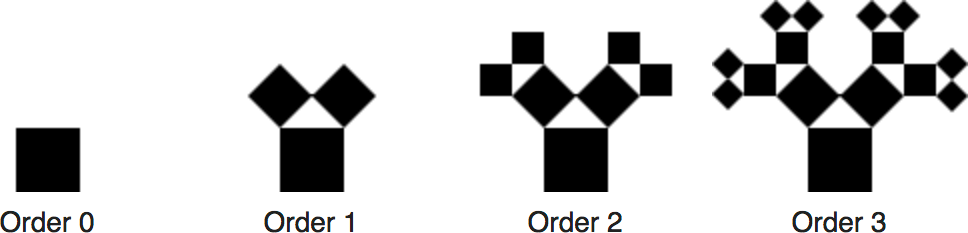
\includegraphics[width=0.7\textwidth]{cp1718t_media/pythagoras-tree1.png}
\end{center}
\caption{Passos de construção de uma árvore de Pitágoras de ordem $3$.}
\label{fig:pitagoras1}
\end{figure}

\href{https://en.wikipedia.org/wiki/Fractal}{Fractais} são formas geométricas que podem ser construídas recursivamente de acordo com um conjunto de equações matemáticas.
Um exemplo clássico de um fractal são as \href{https://en.wikipedia.org/wiki/Pythagoras_tree_(fractal)}{árvores de Pitágoras}.
A construção de uma árvore de Pitágoras começa com um quadrado, ao qual se unem dois quadrados redimensionados pela escala $\sqrt{2}/2$, de forma a que os cantos dos $3$ quadrados coincidam e formem um triângulo rectângulo isósceles.
Este procedimento é repetido recursivamente de acordo com uma dada ordem, definida como um número natural (Figura~\ref{fig:pitagoras1}).

Uma árvore de Pitágoras pode ser codificada em Haskell como uma full tree contendo quadrados nos nodos e nas folhas, sendo um quadrado definido simplesmente pelo tamanho do seu lado:
\begin{hscode}\SaveRestoreHook
\column{B}{@{}>{\hspre}l<{\hspost}@{}}%
\column{E}{@{}>{\hspre}l<{\hspost}@{}}%
\>[B]{}\mathbf{data}\;\Conid{FTree}\;\Varid{a}\;\Varid{b}\mathrel{=}\Conid{Unit}\;\Varid{b}\mid \Conid{Comp}\;\Varid{a}\;(\Conid{FTree}\;\Varid{a}\;\Varid{b})\;(\Conid{FTree}\;\Varid{a}\;\Varid{b})\;\mathbf{deriving}\;(\Conid{Eq},\Conid{Show}){}\<[E]%
\\
\>[B]{}\mathbf{type}\;\Conid{PTree}\mathrel{=}\Conid{FTree}\;\Conid{Square}\;\Conid{Square}{}\<[E]%
\\
\>[B]{}\mathbf{type}\;\Conid{Square}\mathrel{=}\Conid{Float}{}\<[E]%
\ColumnHook
\end{hscode}\resethooks

\begin{enumerate}
    \item Defina a função \ensuremath{\Varid{generatePTree}\mathbin{::}\Conid{Int}\to \Conid{PTree}}, como um anamorfismo, que gera uma árvore de Pitágoras para uma dada ordem.


\begin{propriedade}
    Uma árvore de Pitágoras tem profundidade igual à sua ordem:
\begin{hscode}\SaveRestoreHook
\column{B}{@{}>{\hspre}l<{\hspost}@{}}%
\column{E}{@{}>{\hspre}l<{\hspost}@{}}%
\>[B]{}\Varid{prop4a}\;(\Conid{SmallNat}\;\Varid{n})\mathrel{=}(\Varid{depthFTree}\comp \Varid{generatePTree})\;\Varid{n}\equiv \Varid{n}{}\<[E]%
\ColumnHook
\end{hscode}\resethooks
\end{propriedade}
\begin{propriedade}
    Uma árvore de Pitágoras está sempre balanceada:
\begin{hscode}\SaveRestoreHook
\column{B}{@{}>{\hspre}l<{\hspost}@{}}%
\column{E}{@{}>{\hspre}l<{\hspost}@{}}%
\>[B]{}\Varid{prop4b}\;(\Conid{SmallNat}\;\Varid{n})\mathrel{=}(\Varid{isBalancedFTree}\comp \Varid{generatePTree})\;\Varid{n}{}\<[E]%
\ColumnHook
\end{hscode}\resethooks
\end{propriedade}

\item Defina a função \ensuremath{\Varid{drawPTree}\mathbin{::}\Conid{PTree}\to [\mskip1.5mu \Conid{Picture}\mskip1.5mu]}, utilizando catamorfismos e/ou anamorfismos, que anima incrementalmente os passos de construção de uma árvore de Pitágoras recorrendo à biblioteca \href{https://hackage.haskell.org/package/gloss}{gloss}.
    Anime a sua solução:
\begin{tabbing}\ttfamily
~~~~~\char62{}~animatePTree~3
\end{tabbing}

    
\end{enumerate}

\section*{Problema 5}

Uma das áreas em maior expansão no campo da informática é a análise de dados
e  \href{https://www.mathworks.com/discovery/machine-learning.html}{machine learning}. Esta questão aborda um \emph{mónade} que ajuda
a fazer, de forma simples, as operações básicas dessas técnicas. Esse mónade
é conhecido por \emph{bag}, \emph{saco} ou \emph{multi-conjunto}, permitindo
que os elementos de um conjunto tenham multiplicidades associadas. Por exemplo,
seja
\begin{hscode}\SaveRestoreHook
\column{B}{@{}>{\hspre}l<{\hspost}@{}}%
\column{E}{@{}>{\hspre}l<{\hspost}@{}}%
\>[B]{}\mathbf{data}\;\Conid{Marble}\mathrel{=}\Conid{Red}\mid \Conid{Pink}\mid \Conid{Green}\mid \Conid{Blue}\mid \Conid{White}\;\mathbf{deriving}\;(\Conid{Read},\Conid{Show},\Conid{Eq},\Conid{Ord}){}\<[E]%
\ColumnHook
\end{hscode}\resethooks
um tipo dado.\footnote{``Marble" traduz para ``berlinde" em português.}
A lista \ensuremath{[\mskip1.5mu \Conid{Pink},\Conid{Green},\Conid{Red},\Conid{Blue},\Conid{Green},\Conid{Red},\Conid{Green},\Conid{Pink},\Conid{Blue},\Conid{White}\mskip1.5mu]} tem elementos
repetidos. Assumindo que a ordem não é importante, essa lista corresponde ao saco
\begin{quote}\small
\begin{tabbing}\ttfamily
~\char123{}~Red~\char124{}\char45{}\char62{}~2~\char44{}~Pink~\char124{}\char45{}\char62{}~2~\char44{}~Green~\char124{}\char45{}\char62{}~3~\char44{}~Blue~\char124{}\char45{}\char62{}~2~\char44{}~White~\char124{}\char45{}\char62{}~1~\char125{}
\end{tabbing}
\end{quote}
que habita o tipo genérico dos ``bags":
\begin{hscode}\SaveRestoreHook
\column{B}{@{}>{\hspre}l<{\hspost}@{}}%
\column{E}{@{}>{\hspre}l<{\hspost}@{}}%
\>[B]{}\mathbf{data}\;\Conid{Bag}\;\Varid{a}\mathrel{=}\Conid{B}\;[\mskip1.5mu (\Varid{a},\Conid{Int})\mskip1.5mu]\;\mathbf{deriving}\;(\Conid{Ord}){}\<[E]%
\ColumnHook
\end{hscode}\resethooks
O mónade que vamos construir sobre este tipo de dados faz a gestão automática das multiciplidades.
Por exemplo, seja dada a função que dá o peso de cada berlinde em gramas:
\begin{hscode}\SaveRestoreHook
\column{B}{@{}>{\hspre}l<{\hspost}@{}}%
\column{20}{@{}>{\hspre}l<{\hspost}@{}}%
\column{E}{@{}>{\hspre}l<{\hspost}@{}}%
\>[B]{}\Varid{marbleWeight}\mathbin{::}\Conid{Marble}\to \Conid{Int}{}\<[E]%
\\
\>[B]{}\Varid{marbleWeight}\;\Conid{Red}{}\<[20]%
\>[20]{}\mathrel{=}\mathrm{3}{}\<[E]%
\\
\>[B]{}\Varid{marbleWeight}\;\Conid{Pink}{}\<[20]%
\>[20]{}\mathrel{=}\mathrm{2}{}\<[E]%
\\
\>[B]{}\Varid{marbleWeight}\;\Conid{Green}\mathrel{=}\mathrm{3}{}\<[E]%
\\
\>[B]{}\Varid{marbleWeight}\;\Conid{Blue}{}\<[20]%
\>[20]{}\mathrel{=}\mathrm{6}{}\<[E]%
\\
\>[B]{}\Varid{marbleWeight}\;\Conid{White}\mathrel{=}\mathrm{2}{}\<[E]%
\ColumnHook
\end{hscode}\resethooks
Então, se quisermos saber quantos \emph{berlindes} temos, de cada \emph{peso}, não teremos que fazer contas:
basta calcular
\begin{hscode}\SaveRestoreHook
\column{B}{@{}>{\hspre}l<{\hspost}@{}}%
\column{E}{@{}>{\hspre}l<{\hspost}@{}}%
\>[B]{}\Varid{marbleWeights}\mathrel{=}\mathsf{fmap}\;\Varid{marbleWeight}\;\Varid{bagOfMarbles}{}\<[E]%
\ColumnHook
\end{hscode}\resethooks
onde \ensuremath{\Varid{bagOfMarbles}} é o saco de berlindes referido acima, obtendo-se:
\begin{quote}\small
	\text{\ttfamily \char123{}~2~\char124{}\char45{}\char62{}~3~\char44{}~3~\char124{}\char45{}\char62{}~5~\char44{}~6~\char124{}\char45{}\char62{}~2~\char125{}}.
\end{quote}
%
Mais ainda, se quisermos saber o total de berlindes em \ensuremath{\Varid{bagOfMarbles}} basta
calcular \ensuremath{\mathsf{fmap}\;(\mathbin{!})\;\Varid{bagOfMarbles}} obtendo-se \text{\ttfamily \char123{}~\char40{}\char41{}~\char124{}\char45{}\char62{}~10~\char125{}}; isto é,
o saco tem \ensuremath{\mathrm{10}} berlindes no total.


Finalmente, se quisermos saber a probabilidade da cor de um berlinde que tiremos do saco, basta converter
o referido saco numa distribuição correndo:
\begin{hscode}\SaveRestoreHook
\column{B}{@{}>{\hspre}l<{\hspost}@{}}%
\column{E}{@{}>{\hspre}l<{\hspost}@{}}%
\>[B]{}\Varid{marblesDist}\mathrel{=}\Varid{dist}\;\Varid{bagOfMarbles}{}\<[E]%
\ColumnHook
\end{hscode}\resethooks
obtendo-se a distribuição (graças ao módulo \Probability):
\begin{quote}\small
\begin{tabbing}\ttfamily
~Green~~30\char46{}0\char37{}\\
\ttfamily ~~~Red~~20\char46{}0\char37{}\\
\ttfamily ~~Pink~~20\char46{}0\char37{}\\
\ttfamily ~~Blue~~20\char46{}0\char37{}\\
\ttfamily ~White~~10\char46{}0\char37{}
\end{tabbing}
\end{quote}
cf.\ Figura \ref{fig:dist}.

\begin{figure}
\begin{center}
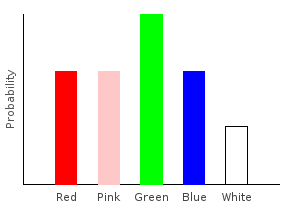
\includegraphics[width=0.4\textwidth]{cp1718t_media/marblesDist-mod5.png}
\end{center}
\caption{Distribuição de berlindes num saco.}
\label{fig:dist}
\end{figure}

Partindo da seguinte declaração de \ensuremath{\Conid{Bag}} como um functor e como um mónade,
\begin{hscode}\SaveRestoreHook
\column{B}{@{}>{\hspre}l<{\hspost}@{}}%
\column{4}{@{}>{\hspre}l<{\hspost}@{}}%
\column{5}{@{}>{\hspre}l<{\hspost}@{}}%
\column{E}{@{}>{\hspre}l<{\hspost}@{}}%
\>[B]{}\mathbf{instance}\;\Conid{Functor}\;\Conid{Bag}\;\mathbf{where}{}\<[E]%
\\
\>[B]{}\hsindent{5}{}\<[5]%
\>[5]{}\mathsf{fmap}\;\Varid{f}\mathrel{=}\Conid{B}\comp \map \;(\Varid{f}\times\Varid{id})\comp \Varid{unB}{}\<[E]%
\\[\blanklineskip]%
\>[B]{}\mathbf{instance}\;\Conid{Monad}\;\Conid{Bag}\;\mathbf{where}{}\<[E]%
\\
\>[B]{}\hsindent{4}{}\<[4]%
\>[4]{}\Varid{x}\bind \Varid{f}\mathrel{=}(\mu \comp \mathsf{fmap}\;\Varid{f})\;\Varid{x}\;\mathbf{where}{}\<[E]%
\\
\>[B]{}\hsindent{4}{}\<[4]%
\>[4]{}\Varid{return}\mathrel{=}\Varid{singletonbag}{}\<[E]%
\ColumnHook
\end{hscode}\resethooks
\begin{enumerate}
\item	
Defina a função \ensuremath{\mu } (multiplicação do mónade \ensuremath{\Conid{Bag}}) e a função auxiliar
\ensuremath{\Varid{singletonbag}}.
\item	Verifique-as com os seguintes testes unitários:
\begin{teste}
Lei \ensuremath{\mu \comp \Varid{return}\mathrel{=}\Varid{id}}:
\begin{hscode}\SaveRestoreHook
\column{B}{@{}>{\hspre}l<{\hspost}@{}}%
\column{E}{@{}>{\hspre}l<{\hspost}@{}}%
\>[B]{}\Varid{test5a}\mathrel{=}\Varid{bagOfMarbles}\equiv \mu \;(\Varid{return}\;\Varid{bagOfMarbles}){}\<[E]%
\ColumnHook
\end{hscode}\resethooks
\end{teste}
\begin{teste}
Lei \ensuremath{\mu \comp \mu \mathrel{=}\mu \comp \mathsf{fmap}\;\mu }:
\begin{hscode}\SaveRestoreHook
\column{B}{@{}>{\hspre}l<{\hspost}@{}}%
\column{E}{@{}>{\hspre}l<{\hspost}@{}}%
\>[B]{}\Varid{test5b}\mathrel{=}(\mu \comp \mu )\;\Varid{b3}\equiv (\mu \comp \mathsf{fmap}\;\mu )\;\Varid{b3}{}\<[E]%
\ColumnHook
\end{hscode}\resethooks
\vskip 1em
onde \ensuremath{\Varid{b3}} é um saco dado em anexo.
\end{teste}
\end{enumerate}

%----------------- Bibliografia (exige bibtex) --------------------------------%

\bibliographystyle{plain}
\bibliography{cp1718t}

%----------------- Programa, bibliotecas e código auxiliar --------------------%

\newpage

\part*{Anexos}

\appendix

\section{Mónade para probabilidades e estatística}\label{sec:Dist}
Mónades são functores com propriedades adicionais que nos permitem obter
efeitos especiais em progra\-mação. Por exemplo, a biblioteca \Probability\
oferece um mónade para abordar problemas de probabilidades. Nesta biblioteca,
o conceito de distribuição estatística é captado pelo tipo
\begin{eqnarray}
	\ensuremath{\mathbf{newtype}\;\fun{Dist}\;\Varid{a}\mathrel{=}\Conid{D}\;\{\mskip1.5mu \Varid{unD}\mathbin{::}[\mskip1.5mu (\Varid{a},\Conid{ProbRep})\mskip1.5mu]\mskip1.5mu\}}
	\label{eq:Dist}
\end{eqnarray}
em que \ensuremath{\Conid{ProbRep}} é um real de \ensuremath{\mathrm{0}} a \ensuremath{\mathrm{1}}, equivalente a uma escala de \ensuremath{\mathrm{0}} a \ensuremath{\mathrm{100}\mathbin{/}}.

Cada par \ensuremath{(\Varid{a},\Varid{p})} numa distribuição \ensuremath{\Varid{d}\mathbin{::}\fun{Dist}\;\Varid{a}} indica que a probabilidade
de \ensuremath{\Varid{a}} é \ensuremath{\Varid{p}}, devendo ser garantida a propriedade de  que todas as probabilidades
de \ensuremath{\Varid{d}} somam \ensuremath{\mathrm{100}\mathbin{/}}.
Por exemplo, a seguinte distribuição de classificações por escalões de $A$ a $E$,
\[
\begin{array}{ll}
A & \rule{2mm}{3pt}\ 2\%\\
B & \rule{12mm}{3pt}\ 12\%\\
C & \rule{29mm}{3pt}\ 29\%\\
D & \rule{35mm}{3pt}\ 35\%\\
E & \rule{22mm}{3pt}\ 22\%\\
\end{array}
\]
será representada pela distribuição
\begin{hscode}\SaveRestoreHook
\column{B}{@{}>{\hspre}l<{\hspost}@{}}%
\column{E}{@{}>{\hspre}l<{\hspost}@{}}%
\>[B]{}\Varid{d1}\mathbin{::}\fun{Dist}\;\Conid{Char}{}\<[E]%
\\
\>[B]{}\Varid{d1}\mathrel{=}\Conid{D}\;[\mskip1.5mu (\text{\ttfamily 'A'},\mathrm{0.02}),(\text{\ttfamily 'B'},\mathrm{0.12}),(\text{\ttfamily 'C'},\mathrm{0.29}),(\text{\ttfamily 'D'},\mathrm{0.35}),(\text{\ttfamily 'E'},\mathrm{0.22})\mskip1.5mu]{}\<[E]%
\ColumnHook
\end{hscode}\resethooks
que o \GHCi\ mostrará assim:
\begin{Verbatim}[fontsize=\small]
'D'  35.0%
'C'  29.0%
'E'  22.0%
'B'  12.0%
'A'   2.0%
\end{Verbatim}

Este mónade é adequado à resolução de problemas de \emph{probabilidades e
estatística} usando programação funcional, de forma elegante e como caso
particular de programação monádica.

\section{Definições auxiliares}\label{sec:helper_functions}
Funções para mostrar \emph{bags}:
\begin{hscode}\SaveRestoreHook
\column{B}{@{}>{\hspre}l<{\hspost}@{}}%
\column{5}{@{}>{\hspre}l<{\hspost}@{}}%
\column{8}{@{}>{\hspre}l<{\hspost}@{}}%
\column{18}{@{}>{\hspre}l<{\hspost}@{}}%
\column{33}{@{}>{\hspre}l<{\hspost}@{}}%
\column{36}{@{}>{\hspre}l<{\hspost}@{}}%
\column{E}{@{}>{\hspre}l<{\hspost}@{}}%
\>[B]{}\mathbf{instance}\;(\Conid{Show}\;\Varid{a},\Conid{Ord}\;\Varid{a},\Conid{Eq}\;\Varid{a})\Rightarrow \Conid{Show}\;(\Conid{Bag}\;\Varid{a})\;\mathbf{where}{}\<[E]%
\\
\>[B]{}\hsindent{5}{}\<[5]%
\>[5]{}\Varid{show}\mathrel{=}\Varid{showbag}\comp \Varid{consol}\comp \Varid{unB}\;{}\<[36]%
\>[36]{}\mathbf{where}{}\<[E]%
\\
\>[5]{}\hsindent{3}{}\<[8]%
\>[8]{}\Varid{showbag}\mathrel{=}\Varid{concat}\comp {}\<[E]%
\\
\>[8]{}\hsindent{10}{}\<[18]%
\>[18]{}(\plus [\mskip1.5mu \text{\ttfamily \char34 ~\char125 \char34}\mskip1.5mu])\comp {}\<[33]%
\>[33]{}(\text{\ttfamily \char34 \char123 ~\char34}\mathbin{:})\comp {}\<[E]%
\\
\>[8]{}\hsindent{10}{}\<[18]%
\>[18]{}(\Varid{intersperse}\;\text{\ttfamily \char34 ~,~\char34})\comp {}\<[E]%
\\
\>[8]{}\hsindent{10}{}\<[18]%
\>[18]{}\Varid{sort}\comp {}\<[E]%
\\
\>[8]{}\hsindent{10}{}\<[18]%
\>[18]{}(\map \;\Varid{f})\;\mathbf{where}\;\Varid{f}\;(\Varid{a},\Varid{b})\mathrel{=}(\Varid{show}\;\Varid{a})\plus \text{\ttfamily \char34 ~|->~\char34}\plus (\Varid{show}\;\Varid{b}){}\<[E]%
\\
\>[B]{}\Varid{unB}\;(\mathit B\;\Varid{x})\mathrel{=}\Varid{x}{}\<[E]%
\ColumnHook
\end{hscode}\resethooks
Igualdade de \emph{bags}:
\begin{hscode}\SaveRestoreHook
\column{B}{@{}>{\hspre}l<{\hspost}@{}}%
\column{4}{@{}>{\hspre}l<{\hspost}@{}}%
\column{12}{@{}>{\hspre}l<{\hspost}@{}}%
\column{18}{@{}>{\hspre}l<{\hspost}@{}}%
\column{E}{@{}>{\hspre}l<{\hspost}@{}}%
\>[B]{}\mathbf{instance}\;(\Conid{Eq}\;\Varid{a})\Rightarrow \Conid{Eq}\;(\Conid{Bag}\;\Varid{a})\;\mathbf{where}{}\<[E]%
\\
\>[B]{}\hsindent{4}{}\<[4]%
\>[4]{}\Varid{b}\equiv \Varid{b'}\mathrel{=}(\Varid{unB}\;\Varid{b})\mathbin{`\Varid{lequal}`}(\Varid{unB}\;\Varid{b'}){}\<[E]%
\\
\>[4]{}\hsindent{8}{}\<[12]%
\>[12]{}\mathbf{where}\;\Varid{lequal}\;\Varid{a}\;\Varid{b}\mathrel{=}\Varid{isempty}\;(\Varid{a}\mathbin{\ominus}\Varid{b}){}\<[E]%
\\
\>[12]{}\hsindent{6}{}\<[18]%
\>[18]{}\Varid{ominus}\;\Varid{a}\;\Varid{b}\mathrel{=}\Varid{a}\plus \Varid{neg}\;\Varid{b}{}\<[E]%
\\
\>[12]{}\hsindent{6}{}\<[18]%
\>[18]{}\Varid{neg}\;\Varid{x}\mathrel{=}[\mskip1.5mu (\Varid{k},\mathbin{-}\Varid{i})\mid (\Varid{k},\Varid{i})\leftarrow \Varid{x}\mskip1.5mu]{}\<[E]%
\ColumnHook
\end{hscode}\resethooks
Ainda sobre o mónade \ensuremath{\Conid{Bag}}:
\begin{hscode}\SaveRestoreHook
\column{B}{@{}>{\hspre}l<{\hspost}@{}}%
\column{5}{@{}>{\hspre}l<{\hspost}@{}}%
\column{E}{@{}>{\hspre}l<{\hspost}@{}}%
\>[B]{}\mathbf{instance}\;\Conid{Applicative}\;\Conid{Bag}\;\mathbf{where}{}\<[E]%
\\
\>[B]{}\hsindent{5}{}\<[5]%
\>[5]{}\Varid{pure}\mathrel{=}\Varid{return}{}\<[E]%
\\
\>[B]{}\hsindent{5}{}\<[5]%
\>[5]{}(\mathbin{<*>})\mathrel{=}\Varid{aap}{}\<[E]%
\ColumnHook
\end{hscode}\resethooks
O exemplo do texto:
\begin{hscode}\SaveRestoreHook
\column{B}{@{}>{\hspre}l<{\hspost}@{}}%
\column{E}{@{}>{\hspre}l<{\hspost}@{}}%
\>[B]{}\Varid{bagOfMarbles}\mathrel{=}\mathit B\;[\mskip1.5mu (\Conid{Pink},\mathrm{2}),(\Conid{Green},\mathrm{3}),(\Conid{Red},\mathrm{2}),(\Conid{Blue},\mathrm{2}),(\Conid{White},\mathrm{1})\mskip1.5mu]{}\<[E]%
\ColumnHook
\end{hscode}\resethooks
Um valor para teste (bags de bags de bags):
\begin{hscode}\SaveRestoreHook
\column{B}{@{}>{\hspre}l<{\hspost}@{}}%
\column{7}{@{}>{\hspre}l<{\hspost}@{}}%
\column{E}{@{}>{\hspre}l<{\hspost}@{}}%
\>[B]{}\Varid{b3}\mathbin{::}\Conid{Bag}\;(\Conid{Bag}\;(\Conid{Bag}\;\Conid{Marble})){}\<[E]%
\\
\>[B]{}\Varid{b3}\mathrel{=}\mathit B\;[\mskip1.5mu (\mathit B\;[\mskip1.5mu (\mathit B\;[\mskip1.5mu (\Conid{Pink},\mathrm{2}),(\Conid{Green},\mathrm{3}),(\Conid{Red},\mathrm{2}),(\Conid{Blue},\mathrm{2}),(\Conid{White},\mathrm{1})\mskip1.5mu],\mathrm{5}){}\<[E]%
\\
\>[B]{}\hsindent{7}{}\<[7]%
\>[7]{},(\mathit B\;[\mskip1.5mu (\Conid{Pink},\mathrm{1}),(\Conid{Green},\mathrm{2}),(\Conid{Red},\mathrm{1}),(\Conid{Blue},\mathrm{1})\mskip1.5mu],\mathrm{2})\mskip1.5mu],\mathrm{2})\mskip1.5mu]{}\<[E]%
\ColumnHook
\end{hscode}\resethooks
Outras funções auxiliares:
\begin{hscode}\SaveRestoreHook
\column{B}{@{}>{\hspre}l<{\hspost}@{}}%
\column{E}{@{}>{\hspre}l<{\hspost}@{}}%
\>[B]{}\Varid{a}\mapsto\Varid{b}\mathrel{=}(\Varid{a},\Varid{b}){}\<[E]%
\\[\blanklineskip]%
\>[B]{}\Varid{consol}\mathbin{::}(\Conid{Eq}\;\Varid{b})\Rightarrow [\mskip1.5mu (\Varid{b},\Conid{Int})\mskip1.5mu]\to [\mskip1.5mu (\Varid{b},\Conid{Int})\mskip1.5mu]{}\<[E]%
\\
\>[B]{}\Varid{consol}\mathrel{=}\Varid{filter}\;\Varid{nzero}\comp \map \;(\Varid{id}\times\Varid{sum})\comp \Varid{col}\;\mathbf{where}\;\Varid{nzero}\;(\anonymous ,\Varid{x})\mathrel{=}\Varid{x}\not\equiv \mathrm{0}{}\<[E]%
\\[\blanklineskip]%
\>[B]{}\Varid{isempty}\mathbin{::}\Conid{Eq}\;\Varid{a}\Rightarrow [\mskip1.5mu (\Varid{a},\Conid{Int})\mskip1.5mu]\to \Conid{Bool}{}\<[E]%
\\
\>[B]{}\Varid{isempty}\mathrel{=}\Varid{all}\;(\equiv \mathrm{0})\comp \map \;\p2\comp \Varid{consol}{}\<[E]%
\\[\blanklineskip]%
\>[B]{}\Varid{col}\;\Varid{x}\mathrel{=}\Varid{nub}\;[\mskip1.5mu \Varid{k}\mapsto[\mskip1.5mu \Varid{d'}\mid (\Varid{k'},\Varid{d'})\leftarrow \Varid{x},\Varid{k'}\equiv \Varid{k}\mskip1.5mu]\mid (\Varid{k},\Varid{d})\leftarrow \Varid{x}\mskip1.5mu]{}\<[E]%
\\[\blanklineskip]%
\>[B]{}\Varid{consolidate}\mathbin{::}\Conid{Eq}\;\Varid{a}\Rightarrow \Conid{Bag}\;\Varid{a}\to \Conid{Bag}\;\Varid{a}{}\<[E]%
\\
\>[B]{}\Varid{consolidate}\mathrel{=}\mathit B\comp \Varid{consol}\comp \Varid{unB}{}\<[E]%
\ColumnHook
\end{hscode}\resethooks

%----------------- Soluções dos alunos -----------------------------------------%

\section{Soluções dos alunos}\label{sec:resolucao}
Os alunos devem colocar neste anexo as suas soluções aos exercícios
propostos, de acordo com o ``layout'' que se fornece. Não podem ser
alterados os nomes ou tipos das funções dadas, mas pode ser adicionado texto e / ou 
outras funções auxiliares que sejam necessárias.

\subsection*{Problema 1}

\begin{hscode}\SaveRestoreHook
\column{B}{@{}>{\hspre}l<{\hspost}@{}}%
\column{E}{@{}>{\hspre}l<{\hspost}@{}}%
\>[B]{}\Varid{inBlockchain}\mathrel{=}\bot {}\<[E]%
\\
\>[B]{}\Varid{outBlockchain}\mathrel{=}\bot {}\<[E]%
\\
\>[B]{}\Varid{recBlockchain}\mathrel{=}\bot {}\<[E]%
\\
\>[B]{}\Varid{cataBlockchain}\mathrel{=}\bot {}\<[E]%
\\
\>[B]{}\Varid{anaBlockchain}\mathrel{=}\bot {}\<[E]%
\\
\>[B]{}\Varid{hyloBlockchain}\mathrel{=}\bot {}\<[E]%
\\[\blanklineskip]%
\>[B]{}\Varid{allTransactions}\mathrel{=}\bot {}\<[E]%
\\
\>[B]{}\Varid{ledger}\mathrel{=}\bot {}\<[E]%
\\
\>[B]{}\Varid{isValidMagicNr}\mathrel{=}\bot {}\<[E]%
\ColumnHook
\end{hscode}\resethooks


\subsection*{Problema 2}

\begin{hscode}\SaveRestoreHook
\column{B}{@{}>{\hspre}l<{\hspost}@{}}%
\column{5}{@{}>{\hspre}l<{\hspost}@{}}%
\column{E}{@{}>{\hspre}l<{\hspost}@{}}%
\>[B]{}\Varid{inQTree}\mathrel{=}\bot {}\<[E]%
\\
\>[B]{}\Varid{outQTree}\mathrel{=}\bot {}\<[E]%
\\
\>[B]{}\Varid{baseQTree}\mathrel{=}\bot {}\<[E]%
\\
\>[B]{}\Varid{recQTree}\mathrel{=}\bot {}\<[E]%
\\
\>[B]{}\Varid{cataQTree}\mathrel{=}\bot {}\<[E]%
\\
\>[B]{}\Varid{anaQTree}\mathrel{=}\bot {}\<[E]%
\\
\>[B]{}\Varid{hyloQTree}\mathrel{=}\bot {}\<[E]%
\\[\blanklineskip]%
\>[B]{}\mathbf{instance}\;\Conid{Functor}\;\Conid{QTree}\;\mathbf{where}{}\<[E]%
\\
\>[B]{}\hsindent{5}{}\<[5]%
\>[5]{}\mathsf{fmap}\mathrel{=}\bot {}\<[E]%
\\[\blanklineskip]%
\>[B]{}\Varid{rotateQTree}\mathrel{=}\bot {}\<[E]%
\\
\>[B]{}\Varid{scaleQTree}\mathrel{=}\bot {}\<[E]%
\\
\>[B]{}\Varid{invertQTree}\mathrel{=}\bot {}\<[E]%
\\
\>[B]{}\Varid{compressQTree}\mathrel{=}\bot {}\<[E]%
\\
\>[B]{}\Varid{outlineQTree}\mathrel{=}\bot {}\<[E]%
\ColumnHook
\end{hscode}\resethooks

\subsection*{Problema 3}

\begin{hscode}\SaveRestoreHook
\column{B}{@{}>{\hspre}l<{\hspost}@{}}%
\column{E}{@{}>{\hspre}l<{\hspost}@{}}%
\>[B]{}\Varid{base}\mathrel{=}\bot {}\<[E]%
\\
\>[B]{}\Varid{loop}\mathrel{=}\bot {}\<[E]%
\ColumnHook
\end{hscode}\resethooks

\subsection*{Problema 4}

\begin{hscode}\SaveRestoreHook
\column{B}{@{}>{\hspre}l<{\hspost}@{}}%
\column{5}{@{}>{\hspre}l<{\hspost}@{}}%
\column{E}{@{}>{\hspre}l<{\hspost}@{}}%
\>[B]{}\Varid{inFTree}\mathrel{=}\bot {}\<[E]%
\\
\>[B]{}\Varid{outFTree}\mathrel{=}\bot {}\<[E]%
\\
\>[B]{}\Varid{baseFTree}\mathrel{=}\bot {}\<[E]%
\\
\>[B]{}\Varid{recFTree}\mathrel{=}\bot {}\<[E]%
\\
\>[B]{}\Varid{cataFTree}\mathrel{=}\bot {}\<[E]%
\\
\>[B]{}\Varid{anaFTree}\mathrel{=}\bot {}\<[E]%
\\
\>[B]{}\Varid{hyloFTree}\mathrel{=}\bot {}\<[E]%
\\[\blanklineskip]%
\>[B]{}\mathbf{instance}\;\Conid{Bifunctor}\;\Conid{FTree}\;\mathbf{where}{}\<[E]%
\\
\>[B]{}\hsindent{5}{}\<[5]%
\>[5]{}\Varid{bimap}\mathrel{=}\bot {}\<[E]%
\\[\blanklineskip]%
\>[B]{}\Varid{generatePTree}\mathrel{=}\bot {}\<[E]%
\\
\>[B]{}\Varid{drawPTree}\mathrel{=}\bot {}\<[E]%
\ColumnHook
\end{hscode}\resethooks

\subsection*{Problema 5}

\begin{hscode}\SaveRestoreHook
\column{B}{@{}>{\hspre}l<{\hspost}@{}}%
\column{E}{@{}>{\hspre}l<{\hspost}@{}}%
\>[B]{}\Varid{singletonbag}\mathrel{=}\bot {}\<[E]%
\\
\>[B]{}\mu \mathrel{=}\bot {}\<[E]%
\\
\>[B]{}\Varid{dist}\mathrel{=}\bot {}\<[E]%
\ColumnHook
\end{hscode}\resethooks

\section{Como exprimir cálculos e diagramas em LaTeX/lhs2tex}
Estudar o texto fonte deste trabalho para obter o efeito:\footnote{Exemplos tirados de \cite{Ol18}.} 
\begin{eqnarray*}
\start
	\ensuremath{\Varid{id}\mathrel{=}\conj{\Varid{f}}{\Varid{g}}}
%
\just\equiv{ universal property }
%
        \ensuremath{\begin{lcbr}\p1\comp \Varid{id}\mathrel{=}\Varid{f}\\\p2\comp \Varid{id}\mathrel{=}\Varid{g}\end{lcbr}}
%
\just\equiv{ identity }
%
        \ensuremath{\begin{lcbr}\p1\mathrel{=}\Varid{f}\\\p2\mathrel{=}\Varid{g}\end{lcbr}}
\qed
\end{eqnarray*}

Os diagramas podem ser produzidos recorrendo à \emph{package} \LaTeX\ 
\href{https://ctan.org/pkg/xymatrix}{xymatrix}, por exemplo: 
\begin{eqnarray*}
\xymatrix@C=2cm{
    \ensuremath{\N_0}
           \ar[d]_-{\ensuremath{\cata{\Varid{g}}}}
&
    \ensuremath{\mathrm{1}\mathbin{+}\N_0}
           \ar[d]^{\ensuremath{\Varid{id}\mathbin{+}\cata{\Varid{g}}}}
           \ar[l]_-{\ensuremath{\mathsf{in}}}
\\
     \ensuremath{\mathit B}
&
     \ensuremath{\mathrm{1}\mathbin{+}\mathit B}
           \ar[l]^-{\ensuremath{\Varid{g}}}
}
\end{eqnarray*}

%----------------- Fim do anexo com soluções dos alunos ------------------------%

%----------------- Índice remissivo (exige makeindex) -------------------------%

\printindex

%----------------- Outras definições auxiliares -------------------------------------------%


%----------------- Fim do documento -------------------------------------------%

\end{document}

